\section{Quantum Error Correction Midterm Review - 23 February 2026}
\subsection{Preliminaries}
Gates: 
\begin{itemize}
    \item Hadamard \begin{quantikz} & \gate{H} &\end{quantikz} $\frac{1}{\sqrt{2}}\begin{pmatrix} 1 & 1 \\ 1 & -1 \end{pmatrix}$
    \item Pauli-X \begin{quantikz} & \gate{X} &\end{quantikz} $\begin{pmatrix} 0 & 1 \\ 1 & 0 \end{pmatrix}$
    \item Pauli-Y \begin{quantikz} & \gate{Y} &\end{quantikz} $\begin{pmatrix} 0 & -i \\ i & 0 \end{pmatrix}$
    \item Pauli-Z \begin{quantikz} & \gate{Z} &\end{quantikz} $\begin{pmatrix} 1 & 0 \\ 0 & -1 \end{pmatrix}$
    \item Phase \begin{quantikz} & \gate{S} &\end{quantikz} $\begin{pmatrix} 1 & 0 \\ 0 & i \end{pmatrix}$
    \item $\pi/8$ \begin{quantikz} & \gate{T} &\end{quantikz} $\begin{pmatrix} 1 & 0 \\ 0 & e^{i\pi/4} \end{pmatrix}$
\end{itemize}
Matrix Multiplications:
\begin{itemize}
    \item $X\ket{0} = \ket{1}, X\ket{1} = \ket{0}$, $Y\ket{0} = i\ket{1}, Y\ket{1} = -i\ket{0}$, $Z\ket{0} = \ket{0}, Z\ket{1} = -\ket{1}$
    \item $HXH = Z$, $HZH = X$, $HYH = -Y$
    \item $SXS^\dagger = Y$, $SYS^\dagger = X$, $SZS^\dagger = Z$   
\end{itemize}

\subsection{Lecture 1: Introduction, Quantum Circuits and Density Matrices}

\subsection{Introduction}
Quantum Mechanics Postulates: 1) States: Quantum system = unit vector $=k\ket{\psi}$, 2) Gates: $\ket{\psi'} = U\ket{\psi}$, 3) Measurement: collection of $\{M_m\}$ of measurement operators. The index $m$ refers to the measurement outcomes, probability is given by $p(m) = \braket{\psi|M_k|\psi}$ , 4) Composition: Tensor Product (many qubits)  \\


\subsubsection{Quantum Circuits, Density Matrices}
Density matrices: Suppose we have $\ket{\psi}$ or $\ket{\phi} $ with probability $\frac{1}{2}$? The density matrix is given by $\rho = \frac{1}{2} \ketbra{\psi} + \frac{1}{2} \phi$. \\

Suppose
\begin{quantikz}
    \makeebit{$\ket{\psi}_{AB}$} & \wire[l][1]["A"{above,pos=0.3}]{a} & \rstick{state?} \\
            & \wire[l][1]["B"{above,pos=0.3}]{a}& \meter{}
\end{quantikz}
Let $\ket{\psi}_{AB} = \sqrt{\frac{3}{4}} \ket{00} + \sqrt{\frac{1}{4}} \ket{11}$. Suppose $B$ measures their state, $A$'s state is a statistical mixture: We get either $\sqrt{\frac{3}{4}} \ket{0}$ or $\sqrt{\frac{1}{4}} \ket{1}$. \\
Suppose we now apply a Hadamard to $B$ before we measure. Then the state after the Hadamard is $\frac{1}{\sqrt{2}}[\sqrt{\frac{3}{4}}\ket{0}(\ket{0} + \ket{1}) + \sqrt{\frac{1}{4}}\ket{1}(\ket{0} - \ket{1})].$ When $B$ measures a $\ket{0}$, then $A$ sees $\sqrt{\frac{3}{4}}\ket{0} + \sqrt{\frac{1}{4}}\ket{1}$. When $A$ measures a $\ket{1}$, then $A$ sees $\sqrt{\frac{3}{4}}\ket{0} - \sqrt{\frac{1}{4}}\ket{1}$. \\
These two matrices are the same statistical mixtures by calculating the density matrices. We can use the definition of density matrix:
\begin{equation}
    \rho = \sum_k \ketbra{\psi_k}
\end{equation}

\begin{definition}
    Density matrix $\rho$ is a density matrix iff $\Tr(\rho) = 1$ and $\rho \geq 0$, i.e. $\forall \ket{\phi}$, $\braket{\phi|\rho|\phi} \geq 0$ and is real. 
\end{definition}

\begin{claim}
    \begin{equation}
        \rho = \sum_k \ketbra{\psi_k}
    \end{equation}
    where $p_k$ is a probability distribution. \\
    Proof: $\Tr(\rho) = \sum p_k = 1$, and $\braket{\phi|\rho|\phi} = \braket{\phi|\psi_k}^2 \geq = 0$
\end{claim}

\begin{claim}
    Any $\rho$ can be expressed as stochastic combination of pure states$\sum_k p_k \ketbra{\psi_k}$ \\
    Proof: $\rho$ is positive and thus has a spectral decomposition. $\rho = \sum_k \lambda_k \ketbra{k}$. The trace is $\sum \lambda_k = 1$ where $\lambda$ is a probability distribution and real. 
\end{claim}

\begin{definition}
    $\rho$ is pure iff $\rho = \ketbra{\psi}$, otherwise $\rho$ is mixed
\end{definition}

Is $\rho = \sum_k p_k \rho_k$ a legal density matrix? Yes!

\begin{lemma}
    von Neumann unravellings: \\
    Let $\rho = \sum_k p_k \ketbra{\psi_k}$. Then $\rho = \rho' = q_k \ketbra{\phi_k}$ if 
    \begin{equation}
        \sqrt{p_k} \ket{\psi_k} = \sum_j U_{kj}\sqrt{q_j}\ket{\phi_j}
    \end{equation}
    (doesn't matter what basis $B$ measures in)
\end{lemma}

\begin{definition}
    A purification of $\rho_A$ is a state $\ket{\psi_{AB}}$ s.t. 
    \begin{equation}
        \rho_A = \Tr_B \ketbra{\psi_{AB}}
    \end{equation}
    where $\Tr_B$ is the partial trace (can be viewed as the circuit earlier. 
\end{definition}


\subsection{Lecture 2: Quantum Operations}
\subsubsection{System-environment model}
Goal: describe all ways in which an $\rho_{in} \xrightarrow{\mathcal{E}} \rho_{out}$, where $\mathcal{E}$ is a map. \\
Model: Suppose 
\begin{center}
\begin{quantikz}
    \lstick{$\ket{\psi}$} & \gate[2]{U} & \rstick{$\rho_{out}$? } \\
    \lstick{$\ket{e}$} &  & \meter{}
\end{quantikz} 
\end{center}
where $\ket{e}$ is the environment and the meter is the is the measurement operators $\ketbra{e_0}, \ketbra{e_1}, \ldots$. \\
\begin{equation}
    \ket{e}\ket{\psi} \rightarrow U \ket{e}\ket{\psi}
\end{equation}
Let $\oplus$ be ``or". Then:
\begin{align}
    \rho &= \braket{e_0|U|e} \oplus \braket{e_1|U|e} \oplus \cdots \\
    &= \oplus_k \braket{e_k|U|e} \ket{\psi}
\end{align}
$E_r = \braket{e_k|U|e}$ is called an ``operation element" or a Krauss operator, or error operator.
\begin{equation}
    \rho_{out} = \sum_k E_k \rho E_k^\dagger = \mathcal{E}(\rho) \quad \text{where } \sum_k E_kE_k^\dagger = I 
\end{equation}
This setup with the system-environment model giving us an equation that maps the input density matrix with an output density matrix is important idea for quantum error correction. 

\subsubsection{Quantum operations - definition and criteria}
In general, what is legal $\rho \rightarrow \mathcal{E}(\rho)$? 
\begin{definition}
    $\mathcal{E}$ is a valid quantum operation iff 
    \begin{enumerate}
        \item Trace preserving $\Tr[\mathcal{E}(\rho)] = 1$
        \item Convex and linear: $\mathcal{E}(\sum_k p_k\rho_k) = \sum p_k \mathcal{E}(\rho_k)$ where $p_k$ are probability distribution
        \item Complete positivity: a) if $\rho \geq 0 \Rightarrow \mathcal{E}(\rho) \geq 0$; b) $(I_R \otimes \mathcal{E}_Q)(\rho_{RQ}) \geq 0$ if $\rho_{RQ} \geq 0$
    \end{enumerate}
\end{definition}


\subsubsection{Operator Sum Representation}
\begin{theorem}
    Let 
    \begin{equation}
    \mathcal{E}(\rho) = \sum_k E_k \rho E_k^\dagger = \mathcal{E}(\rho) \quad \text{where } \sum_k E_kE_k^\dagger = I 
\end{equation}
$\mathcal{E}(\rho)$ is a valid quantum operation.
\end{theorem}
Check if this is true. \\
Thus, for all 
\[
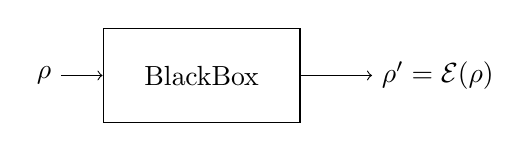
\begin{tikzpicture}[baseline=(current bounding box.center)]
    % Nodes
    \node (rho) at (0,0) {$\rho$};
    \node[draw, minimum width=2.5cm, minimum height=1.2cm] (box) at (2,0) {Black\\Box};
    \node (rho2) at (5,0) {$\rho' = \mathcal{E}(\rho)$};
    
    % Arrows
    \draw[->] (rho) -- (box);
    \draw[->] (box) -- (rho2);
\end{tikzpicture}
\qquad
\text{for some } \{\mathcal{E}_k\}
\]
For all black boxes taking $\rho$ to $\rho' = \mathcal{E}(\rho)$ there will exist a set of quantum operation elements  $\{E_k\}$ to describe any such black box transformation.
Additionally, there exists a system-environment model for any quantum operation $\mathcal{E}$. 
\begin{center}
\begin{quantikz}
    \lstick{$\ket{\psi}$} & \gate[2]{U} & \rstick{$\rho' = \mathcal{E}(\rho)$   } \\
    \lstick{$\ket{e}$} &  & \meter{}
\end{quantikz} 
\end{center}
Due to the fact that we can measure in any basis $E_k$'s are not necessarily unique. 

\begin{example} Operator Sum Representation\\
    \begin{enumerate}
        \item 
        \begin{quantikz}
            & \gate{U} &    
        \end{quantikz} then $\mathcal{E}(\rho) = U\rho U^\dagger$

        \item Let $\{P_k\}$ be projectors
        \begin{quantikz}
            & \meter{} &    
        \end{quantikz} then $\mathcal{E}(\rho) = \sum_k P_k \rho P_k^\dagger$

        \item 
        \begin{quantikz}
            \lstick{$\rho$} & \ctrl{1} & & \rstick{$\mathcal{E}(\rho)$} \\
            \lstick{$\ket{0}$} & \gate{R_y(\theta)} & \meter{}
        \end{quantikz} where the controlled $R_y(\theta)$ is the black box. Recall $R_y = \begin{pmatrix} \cos\frac{\theta}{2} & -\sin\frac{\theta}{2} \\ \sin\frac{\theta}{2} & \cos\frac{\theta}{2} \end{pmatrix}$. Let $\lambda = \sin^2 \frac{\theta}{2}$. Let $e$ be the first qubit and $s$ be the second qubit. Then,
        \begin{equation}
            U = \begin{pmatrix}
                1 & 0 & 0 & 0 \\
                0 & \sqrt{1-\lambda} & 0 & -\lambda \\
                0 & 0 & 1 & 0 \\
                0 & \sqrt{\lambda} & 0 & \sqrt{1-\lambda}
            \end{pmatrix}
        \end{equation}
        Recall $E_k = \braket{e_k|U|e}$. This is not a number but an operator that acts on the system qubit. We can read out of $U$ by looking at the matrix elements that are 0 for the environment qubit which is the upper left box.
        \begin{equation}
            E_0 = \braket{0|U|0} = \begin{pmatrix}1 & 0 \\ 0 & \sqrt{1-\lambda} \end{pmatrix}
        \end{equation}
        similarly, $E_1$ is given by the bottom left matrix. 
        $E_1 = \braket{1|U|0} = \begin{pmatrix}0 & 0 \\ 0 & - \lambda \end{pmatrix}$. \\

        This operation is an important physical process called phase damping. We can see this by applying it to an arbitrary density matrix. 
        \begin{align}
            \mathcal{E}(\rho) &= E_0\rho E_0^\dagger + E_1\rho E_1^\dagger \\
            &= \begin{pmatrix}a & b \\ b^*\sqrt{1-\lambda} & c\sqrt{1-\lambda}\end{pmatrix} E_0^\dagger + \begin{pmatrix}0 & 0 \\ b^* & c\lambda \end{pmatrix} E_1 \\
            &= \begin{pmatrix}a & b\sqrt{1-\lambda} \\ b^*\sqrt{1-\lambda}  & c(1-\lambda)\end{pmatrix} + \begin{pmatrix}0 & 0 \\ 0 & c\lambda \end{pmatrix} \\
            &= \begin{pmatrix}a & b\sqrt{1-\lambda} \\ b^*\sqrt{1-\lambda}  & c\end{pmatrix}
        \end{align}
        If $\sqrt{1-\lambda}$ is an exponentially decaying function in time, often in real practice. $\sqrt{1-\lambda} \rightarrow e^{-t/T_2}$, where $T_2$ is the phase damping time. 

        \item 
        \begin{quantikz}
            \lstick{$\rho$} & \ctrl{1} &  \targ{} &  &\rstick{$\mathcal{E}(\rho)$} \\
            \lstick{$\ket{0}$} & \gate{R_y(\theta)} & \ctrl{-1}& \meter{}
        \end{quantikz} where the controlled $R_y(\theta)$ and controlled-NOT is the black box. \\
        $E_0$ stays the same because the environment does not change only when the system qubit is in the $\ket{0}$ state. The second CNOT does nothing
        \begin{equation}
            E_0 = \braket{0|U|0} = \begin{pmatrix}1 & 0 \\ 0 & \sqrt{1-\lambda} \end{pmatrix}
        \end{equation}
        For $E_1$, the operation element is the same as before, except that an $X$ and not gate has to happen. 
        \begin{equation}
            E_1 = \braket{1|U|0} = \begin{pmatrix} 0 &1 \\ 1 & 0 \end{pmatrix} \begin{pmatrix}0 & 0 \\ 0 & - \lambda \end{pmatrix} = \begin{pmatrix}0 & \sqrt{\lambda} \\ 0 & 0 \end{pmatrix}
        \end{equation}
        This is called amplitude damping. If we apply this to an arbitrary density matrix.
        \begin{equation}
            \mathcal{E}(\rho) = \begin{pmatrix}
                1 - c(1-\lambda) & b\sqrt{1 - \lambda} \\ b^*\sqrt{1-\lambda} & c(1-\lambda) = \begin{pmatrix}
                    1 - ce^{-t/T_1} & b1 - be^{-t/2T_1} \\
                    b^*1 - ce^{-t/2T_1} & ce^{-t/T_1}
                \end{pmatrix}
            \end{pmatrix}
        \end{equation}
        Diagonal decay such that the left top element goes to 1, and the bottom right element goes to 0. Diagonal term decay is the loss of energy of the system, that is the amplitude decay. Note that $T1=2T_2$ which is the loss of energy from a qubit. 
    \end{enumerate}
\end{example}


\subsubsection{Unitary degree of freedom in OSR}
There are infinite choices of $\{E_k\}$ to give the same $\mathcal{E}$.
\begin{center}
\begin{quantikz}
    \lstick{$\ket{\psi}$} & \gate[2]{U} && \rstick{$\rho' = \mathcal{E}(\rho)$   } \\
    \lstick{$\ket{e}$} &  & \gate{U'} & \meter{}
\end{quantikz} 
\end{center}
We can change the basis of the environment before measuring. 
\begin{lemma}
    If $\{E_k\}$ describe a valid operator sum representation $\mathcal{E}$. then $F_j = \sum_k U_{jk}E_k$ describes the same $\mathcal{E}$. \\
    Proof: 
    \begin{equation}
        \sum_j F_j \rho F_j^\dagger = \sum_{jkk'}U_{jk}E_k\rho E_{k'}^\dagger U_{jk'}^* = \sum_{kk'} = \delta_{kk'}E_k\rho E_k^\dagger = \mathcal{E}
    \end{equation}
\end{lemma}


\subsection{Lecture 3: Quantum Error Correction}
\subsubsection{Classical Coding}
Error model: Let the left 0,1 be the sender and the right 0,1 be the receiver. 
\[
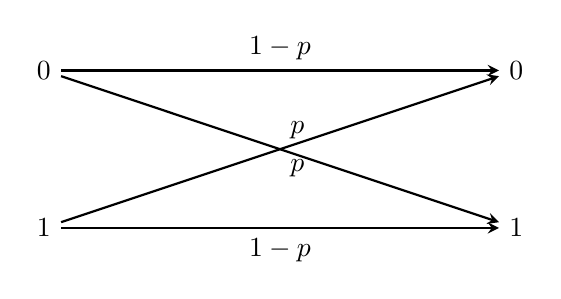
\begin{tikzpicture}[>=stealth, thick]

% Left labels
\node (l0) at (0,2) {$0$};
\node (l1) at (0,0) {$1$};

% Right labels
\node (r0) at (6,2) {$0$};
\node (r1) at (6,0) {$1$};

% Straight arrows (no flip)
\draw[->] (l0) -- node[above] {$1-p$} (r0);
\draw[->] (l1) -- node[below] {$1-p$} (r1);

% Cross arrows (flip)
\draw[->] (l0) -- node[midway, above right] {$p$} (r1);
\draw[->] (l1) -- node[midway, below right] {$p$} (r0);

\end{tikzpicture}
\]
The probability of error is given by $prob(error) = p$. This channel is symmetric and is known as the``binary symmetric channel". 

\begin{definition}
    A classical $[n,k,d]$ code is a set of $2^k$ $n$-bit strings with minimum Hamming distance $d$. 
\end{definition}

\begin{definition}
    $d(x,y) = w(x \oplus y ) = $ Hamming distance where $\oplus$ is bitwise $XOR$ and $w$ is the number of $1$'s (weight)
\end{definition}

\begin{example}
    $000 \rightarrow o_L$ and $111 \rightarrow 1_L$; thus $n=3$, $k=1$, $d=3$. Therefore, $[n,k,d] = [3,1,3]$ \\

    Suppose the sender sends $000 = 0_L$, then apply the binary symmetric channel with probability $p$. What the receiver sees as a result of this error can be written as a stochastic mixture of a certain set of received states
    
    \begin{center}
    \begin{tabular}{ c | c | c }
    Receive & Probability & Decode\\
    \hline
    000 & $(1-p)^3$ & 0 \\
    001 & $p(1-p)^2$ & 0 \\
    010 & $p(1-p)^2$ & 0 \\
    100 & $p(1-p)^2$ & 1 \\
    011 & $p^2(1-p)$ & 1 \\
    101 & $p^2(1-p)$ & 1 \\
    111 & $p^3$ & 1 \\
    \end{tabular}
    \end{center}
    The last 4 rows show that an error has occurred.\\
    The probability of error is given by
    \begin{align}
        Prob(err) = p^3 + 3p^2(1-p) = 3p^2 + 2p^3 = O(p^2)
    \end{align}
    which is lower than the original channel error probability which had $O(p)$. Thus this is an effective way of correcting errors. 
\end{example}


\subsubsection{Quantum Coding}
Circa 1995: Impossible because
\begin{enumerate}
    \item States collapse when measured
    \item Errors are continuous
    \item No-cloning (no redundancy code)
\end{enumerate}
We now get around it by
\begin{enumerate}
    \item Do not measure state holding quantum info - only measure environment
    \item Orthogonal using entanglement
    \item Orthogonal using entanglement
\end{enumerate}

Quantum bit-flip code: \\
Suppose $\mathcal{E}(\rho) = (1-p)\rho + p X \rho X$ ``bit-flip channel" \\
Schematically, 
\begin{center}
\begin{quantikz}
    \lstick{Alice} & \gate{\mathcal{E}(\rho)} & \rstick{Bob} 
\end{quantikz} 
\end{center}
\begin{definition}
    An $[[n,k]]$ quantum code $C$ is a $k$-qubit subspace of an $n$-qubit Hilbert space. 
\end{definition}
\begin{example}
    $n=3, k=1, \ket{000} = \ket{0_L}, \ket{111} = \ket{1_L}$ \\
    naive way of doing it is $a\ket{0} + b\ket{1} \rightarrow (a\ket{0} + b\ket{1})^{\otimes 3}$ but is not possible due to no cloning theorem. \\
    Returning to $\mathcal{E}(\rho) = (1-p)\rho + P X \rho X$. Let $\psi = a\ket{000} + b\ket{111}$
    \begin{center}
    \begin{tabular}{ c | c}
    Receive & Probability \\
    \hline
    $a\ket{000} + b\ket{111}$ & $(1 -p)^3$  \\  
    $a\ket{001} + b\ket{110}$ & $p(1-p)^2$  \\  
    $a\ket{010} + b\ket{101}$ & $p(1-p)^2$  \\  
    $a\ket{100} + b\ket{001}$ & $p(1-p)^2$  \\  
    $a\ket{011} + b\ket{100}$ & $p^2(1-p)$  \\  
    $a\ket{101} + b\ket{010}$ & $p^2(1-p)$  \\  
    $a\ket{100} + b\ket{001}$ & $p^2(1-p)$  \\  
    $a\ket{111} + b\ket{000}$ & $p^3$ 
    \end{tabular}
    \end{center}
    The last 4 states, and error has occurred. The first 4 states are mutually orthogonal, so in principle distinguishable. Error correction should be possible by projecting it onto these orthogonal subspace
\end{example}


\subsubsection{Operator measurement and error syndromes}
Given $U$ has eigenvalues $\pm 1$, and eigenvectors $\ket{\pm U}$, ``measuring U" is: \\
\begin{quantikz}
    \lstick{$\ket{0}$} & \gate{H} \slice{$\phi_0$}& \ctrl{1} \slice{$\phi_1$}& \gate{H} \slice{$\phi_2$}& \meter{Z} \\
    \lstick{$c_0\ket{u_+} + c_1 \ket{u_-}$} & & \gate{U} & & \rstick{$\ket{\psi}$}
\end{quantikz}
\begin{align}
    \ket{\phi_0} &= \frac{\ket{0} + \ket{1}}{\sqrt{2}}[c_0 \ket{u_+} + c_1 \ket{u_-}] \\
    \ket{\phi_1} &=  \frac{\ket{0}}{\sqrt{2}}[c_0 \ket{u_+} + c_1 \ket{u_-}] + \frac{\ket{1}}{\sqrt{2}}[c_0 \ket{u_+} - c_1 \ket{u_-}] \\
    \ket{\phi_2} &=  \frac{\ket{0} + \ket{1}}{\sqrt{2}}[c_0 \ket{u_+} + c_1 \ket{u_-}] + \frac{\ket{0}-\ket{1}}{\sqrt{2}}[c_0 \ket{u_+} - c_1 \ket{u_-}] \\
     &=  \ket{0}c_0 \ket{u_0} + \ket{1} c_1 \ket{u_-}
\end{align}
If we measure $Z=0$, the state is $\ket{\psi} = \ket{u_+}$, and if we measure $Z =1$, the state is $\ket{\psi} = \ket{u_-}$\\



Error correction and Syndrome Measurements

Operation measurement is thus seen as a projector into the $\pm 1$ eigenvalue subspaces of a unitary operator. This is extremely useful for error. Specifically, we will employ operator measurement to obtain the error syndrome. The error syndrome tells us what error has occurred, that is the effect of the environment will be determined by syndrome operators. 

\begin{enumerate}
    \item measure ``syndrome" ops\\
    For the 3-qubit bit-flip code, these are the two syndrome operators: $U_1 = ZZI$ and $U_2 = IZZ$ \\
    Recall the measurement results obtained when the syndrome operators are measured: $ZZI\ket{000} = + \ket{000}$ and $ZZI\ket{111} = (-1 \ket{1})(-1\ket{1})\ket{1}= + \ket{111}$ Therefore, $U_1(a\ket{000} + \ket{b}\ket{111}) = \ket{a}\ket{000} + b\ket{111}$ which has a $+1$ eigenstate which means $m=0$. $U_2\ket{001} = IZZ \ket{001} = -\ket{001}$, $U_2\ket{110} = -\ket{110}$ \\
    We can make the following statement:
    \begin{equation}
        ZZ\ket{xy} = \begin{cases}
            \ket{xy} \text{ if even \#1's} \\
            -\ket{xy} \text{ if odd \#1's} \\
        \end{cases}
    \end{equation}
    Therefore, $U_2(a\ket{001} + \ket{b}\ket{110}) =  -(\ket{a}\ket{001} + b\ket{110})$

\begin{center}
    \begin{tabular}{ c | c | c | c | c | c}
    Receive & Probability & $U_1=ZZI$ & $U_2=IZZ$ & Recovery $R$ & State\\
    \hline
    $a\ket{000} + b\ket{111}$ & $(1 -p)^3$ & 0 & 0 & $I$ & $a\ket{000} + b\ket{111}$\\  
    $a\ket{001} + b\ket{110}$ & $p(1-p)^2$ & 0 & 1 & $X_3$ &$ a\ket{000} + b\ket{111}$\\ 
    $a\ket{010} + b\ket{101}$ & $p(1-p)^2$ & 1 & 1 & $X_2$ & $a\ket{000} + b\ket{111}$\\
    $a\ket{100} + b\ket{001}$ & $p(1-p)^2$ & 1 & 0 & $X_1$ & $a\ket{000} + b\ket{111}$ \\
    $a\ket{011} + b\ket{100}$ & $p^2(1-p)$ & 0 & 1 & $X_3$ & $a\ket{111} + b\ket{000}$\\
    $a\ket{101} + b\ket{010}$ & $p^2(1-p)$ & 1 & 1 & $X_2$ & $a\ket{111} + b\ket{000}$\\
    $a\ket{100} + b\ket{001}$ & $p^2(1-p)$ & 1 & 0 & $X_1$ & $a\ket{111} + b\ket{000}$\\
    $a\ket{111} + b\ket{000}$ & $p^3$ & 0 & 0 & $I$ & $a\ket{111} + b\ket{000}$
    \end{tabular}
\end{center}
\item Apply unitary ``recovery operation" $R$\\ 
$R$ conditioned on syndrome. The result of this recover operation recovers original qubit. This is for single qubit errors. \\

If two errors occurred, we can also get the syndrome measurements. We then get the inverted qubit
$a\ket{111} + b\ket{000}$, the wrong state. \\
    
\end{enumerate}

How good is the error corrected state?:\\
Fidelity: $F= \rho, \ket{\psi}^2 = \braket{\psi|\rho|\psi} \geq 1 -3p^2(1-p) - p^3 = 1 - 3p^2 + 2p^3 = 1 - O(p^2)$. Without quantum error correction this fidelity would have gone as $1-O(p)$. This is a significant improvement, and this is a signature of quantum error correction. \\

Three qubit bit-flip QEC example overall circuit: \\
\begin{center}
\begin{quantikz}
 \wireoverride{n} &  \wireoverride{n} & \wireoverride{n} & \wireoverride{n} \lstick{$\ket{0}$} & \gate{H} & \ctrl{1} & \ctrl{2} & \gate{H} & \meter{m_0} & \cw & \cwbend{1} \\ 
\lstick{$a\ket{0} + b\ket{1}$} & \ctrl{1}  & \ctrl{2} & \gate{\mathcal{E}_{BF}} & \qw  & \gate{Z} & \qw  & \qw  & \qw & \qw & \gate[wires=3]{R} & \qw \\
\lstick{$\ket{0}$} & \targ{} &\qw & \gate{\mathcal{E}_{BF}} & \qw & \qw & \gate{Z} & \gate{Z} & \qw  &\qw  & & \qw \\
\lstick{$\ket{0}$} &   \qw & \targ{} & \gate{\mathcal{E}_{BF}} & \qw & \gate{Z} & \qw & \qw & \qw  & \qw & & \qw \\
 \wireoverride{n} &  \wireoverride{n} & \wireoverride{n} & \wireoverride{n} \lstick{$\ket{0}$} & \gate{H} & \ctrl{-1} & \qw & \ctrl{-2} & \gate{H} & \meter{m_1} & \cwbend{-1} \\ 
\end{quantikz}
\end{center}
The output is $a\ket{000} + b\ket{111}$ with high fidelity. \\

\begin{claim}
    This scheme can also correct a small rotation error! \\
    Proof: $\mathcal{E}(\rho) = e^{-i \epsilon X_1} \rho e^{i \epsilon X_1}$, where $e^{-i \epsilon X_1} = R_{x1}(2\epsilon)$. Then $\mathcal{E}\ket{\psi} = R_{x1}(2\epsilon) \ket{\psi} \simeq \ket{\psi} - i \epsilon X_1 \ket{\psi}$. When no error correction is applied, the fidelity of this output is is the overlap $F = \sqrt{\norm{\braket{\psi|\psi'}}^2} \geq 1- \epsilon$. When error correction is applied, something different happens due to the syndrome measurement. The syndrome measurement causes the superposition of error or no error to collapse. Thus we obtain $\ket{\psi}$ or $-i\epsilon X_1 \ket{\psi}$ where $\epsilon X$ has a bit flip error applied to it. There is no continuous error cases. We either have error or no error and thus the recovery operator applied to the error channel output state gives us a fidelity which to leading error gives us $F(R(\mathcal{E}(\ket{\psi}))) \geq \sqrt{1 - \epsilon^4} \simeq 1 - \epsilon^2$. This is the same improvement as the full quantum error correction circuit. Therefore, the scheme corrects for a small rotation error. 
\end{claim}




\subsubsection{Correcting quantum errors}
Bit flip channel: $\mathcal{E}_{bf}(\rho) = (1-p)\rho + pX\rho X$ ``classical" errors\\ 
Phase flip channel: $\mathcal{E}_{pf}(\rho) = (1-p)\rho + pZ\rho Z$ quantum! \\

Review the bit-flip code: the code word is $\ket{\psi} = a\ket{000} + b\ket{111} = a\ket{0_L} + b\ket{1_L}$. How do we correct phase errors. Recall $H = \frac{1}{\sqrt{2}} = \begin{pmatrix} 1 & 1 \\ 1 & -1 \end{pmatrix}$, $HXH=Z$, and $HZH = X$. Thus
\begin{equation}
    H \mathcal{E}_{bf}(H\rho H) H = \mathcal{E}_{pf}
\end{equation}
Let $\ket{\pm} = \frac{\ket{0} \pm \ket{1}}{\sqrt{2}}$. The the phase flip code is 
\begin{equation}
    \ket{\psi} = c_1 \ket{+++} + b\ket{---}
\end{equation}
where $\ket{+++} = \ket{0_L}$ and $\ket{---} = \ket{1_L}$. Note that $\mathcal{E}_{pf}: \ket{-} \Leftrightarrow \ket{+}$. \\
Phase flip circuit: 
\begin{center}
    \begin{quantikz}
        \lstick{$a\ket{0}+ b\ket{1}$} & \ctrl{1} & \ctrl{2} & \gate{H} & \gate[3]{\mathcal{E}_{pf}}^{\otimes 3} & \gate{H} & \\
        \lstick{$\ket{0}$} & \targ{} & & \gate{H} & & \gate{H} & \rstick{......}\\
        \lstick{$\ket{0}$} &  & \targ{} & \gate{H} & &\gate{H} & 
    \end{quantikz}
\end{center}
Where the circuit is the same syndrome measurements and recovery operations as we did for the 3-qubit bit flip code. 
\begin{claim}
    Arbitrary qubit errors can be represented as $X$, $Z$, $XZ$ errors. \\
    Proof: Recall $\mathcal{E}(\rho) = \sum_k E_k \rho E_k^\dagger$. Recall $Y = \begin{pmatrix}
        0 & -i \\ i & 0 
    \end{pmatrix} = i XZ$. Let $\sigma_j = \{I,X,Y,Z\}$ and $E_k = \sum_j c_{jk}\sigma_j$. Then 
    \begin{equation}
        \mathcal{E}(\rho) = \sum_{kjj'} c_{kj}c_{kj'} \sigma_j \rho \sigma_{j'} = \sum_{jj'} \sigma_j \rho \sigma_{j'}
    \end{equation}
\end{claim}

\begin{example}
    Recall $R_x(2\epsilon) \ket{\psi} \simeq \ket{\psi} - i \epsilon X \ket{\psi}$. Then 
    \begin{equation}
        \mathcal{E}(\rho) = \rho - i\epsilon(X\rho - \rho X) + \epsilon^2 X\rho X
    \end{equation}
    The second term disappears in the syndrome measurement. In particular, what the syndrome measurement does in general removes all these off-diagonal terms in the $\chi$ matrix representation. The syndrome measurement projects the environment into a definite action given action by Pauli matrix namely, $\{X,Y,Z\}$ as the error
\end{example}


\subsubsection{Shor's 9-qubit code}
Codewords for Shor's 9-qubit code:
\begin{align}
    \ket{0_L} & = \frac{(\ket{000} + \ket{111})^{\otimes 3}}{\sqrt{8}} \\
    \ket{1_L} & = \frac{(\ket{000} - \ket{111})^{\otimes 3}}{\sqrt{8}}
\end{align}
This code can correct for any single qubit error. \\
Syndromes and recovery procedure:
\begin{align}
    \ket{0_L} & = (\ket{0_10_20_3} + \ket{1_11_21_3})(\ket{0_40_50_6} + \ket{1_41_51_6})(\ket{0_70_80_9} + \ket{1_71_81_9}) \\
    \ket{1_L} & = (\ket{0_10_20_3} - \ket{1_11_21_3})(\ket{0_40_50_6} - \ket{1_41_51_6})(\ket{0_70_80_9} - \ket{1_71_81_9}) 
\end{align}

For the bit-flip errors: 
\begin{align}
    Z_1Z_2 &\quad Z_2Z_3\\ 
    Z_4Z_5 &\quad Z_5Z_6\\ 
    Z_7Z_8 &\quad Z_8Z_9 
\end{align}
Phase-flip errors:
\begin{align}
    X_1X_2X_3X_4X_5X_6 \\
    X_4X_5X_6X_7X_8X_9
\end{align}
For bit flips, the parity check operators check the pairs of all possible qubits in each one of these triplets for errors. Why are there 3 copies? This is evident from phase flip operators. For phase flips it checks for sign parity between the pairs. 9-qubit code concatenates a bit flip code and a phase flip code. \\

Performance:\\
\# of possible errors: Identity + ($X,Y,Z$ and 9 qubits) $ = 1 + 3\cdot 9 = 28$\\
\# of possible syndrome values: we have 6 possible bit flip syndrome values, and 2 possible phase flip values.,Thus we have $2^8 = 256$ distinguishable errors. Thus, this code can correct some two qubit errors! 

\begin{definition}
    A perfect $[[n,k]]$ code has $\log_2(1+3n)$ syndrome operators.
\end{definition}
\begin{example}
    $[[5,1]]$ code. There are $1 + 3\cdot 5 = 16$ errors, and we have 4 syndrome errors, thus we have $2^4 = 16$ syndrome values. Thus the 5 qubit code is perfect. 
\end{example}



\subsection{Lecture 4: Stabilizer and CSS codes}
\subsubsection{Quantum Error Correction Criteria}
Quantum Error Correction Criteria:\\
Let the channel be $\mathcal{E}(\rho) = \sum_k E_k \rho E_k^\dagger$. 
\begin{theorem}
    Let $C$ be a quantum code defined by the projector $P = \sum_l \ketbra{\psi_l}$. There exists a quantum operation, a recovery and syndrome measurement $R$ which corrects a certain set of errors defined by $\mathcal{E}$ on the subspace $C$ iff 
    \begin{equation}
        PE_k^\dagger E_j P = d \delta_{jk} P
    \end{equation}
    $E_k^\dagger E_j $ denotes the relationship of the two errors $E_k$ and $E_j$. \\
    Equivalently, 
    \begin{equation}
        \braket{\psi_l|E_j^\dagger E_k|\psi_l} = 0, \forall j \neq k, \forall l 
    \end{equation}
    The off-diagonal terms talk about $E_j$ and $E_k$ and say they must be orthogonal for all errors which are different from each other and for all codeword states. This is the \textbf{orthogonality} criterial. For the on-diagonal element 
    \begin{equation}
        \braket{\psi_l|E_k^\dagger E_k|\psi_l} = d_k, \forall l
    \end{equation}
    That is, it must not distinguish codewords. This is the \textbf{non-deformation} criterion. 
\end{theorem}
When these algebraic conditions are satisfied, $R$ exists, and can be also be found using the proof of these conditions. \\
Proof: Intuition: There's a Hilbert space with a subset $C$. This codeword space has as its image under error operators $E$ some transform vector space. For example, $E$ may transform to a smaller or displaced version of itself. Another different error may also map $C$ into an image. If that image collides with the image of the first operator $E$, then we cannot distinguish these two images from each other. Collisions like this are ruled out by the orthogonality. If the images. If the images are all orthogonal and thus distinguishable, the second error correction criterion requires that images not be deformed, that is, an error operator cannot differentially change one basis state by a length that is different from how another basis state is changed. That is the non-deformation criterion. \\

The recovery operator should thus distinguish these image subspace and unshrink them to recover the original by polar decomposition. By polar decomposition, each one of the error operators may be written as $E_k P = U_k \sqrt{PE_k^\dagger E_k P}$, where $u_k$ is the phase portion, i.e. the rotation, and the magnitude is portion is $PE_k^\dagger E_k P$. From the error correction criteria, we know that $PE_k^\dagger E_k P = d_k$. Summarizing,
\begin{equation}
    E_kP = U_k \sqrt{PE_k^\dagger E_k P} = \sqrt{d_k}U_k P 
\end{equation}
The two parts of the recovery operation are first a syndrome measurement and second a rescaling. \\
\begin{enumerate}
    \item Syndrome measurement: We want to project into the $k$th image of the code word space. Let $p_k = U_kPu_k^\dagger = \frac{E_kPu_k^\dagger}{\sqrt{d_k}} = \frac{u_kPE_k^\dagger}{\sqrt{d_k}}$ \\
    By QEC Criteria: $PE_k^\dagger E_jP = d_k \delta_{jk} P$, the $P_k$ are orthogonal to each other: 
    \begin{equation}
        \forall k \neq j\! P_kP_j \propto U_kPE_k^\dagger E_jPu_j^\dagger = 0 
    \end{equation}This is expected since we required that the images of $C$ be orthogonal to each other. and $P_k$ project into the image of $C$. \\
    Thus the recovery operator : measure $P_k$ which gives $k$ as the syndrome for the error. \\

    Given the syndrome for the error, we now want to recover the initial state.

    \item Recovery: Perform $U_k^\dagger$ which undoes the rotation caused by $E_k$. 
    \begin{equation}
        R(\rho) = \sum_k U_k^\dagger P_k \rho P_k U_k
    \end{equation}
    The overall recovery operation combines the syndrome measurement $P_k$. The post-syndrome measurement $\rho'= P_k\rho P_k$. \\
    For a state $\ket{\psi} \in C$, 
    \begin{equation}
        U_k^\dagger P_kE_j \ket{\psi} = \ket{\psi}
    \end{equation}
     where $E_j\ket{\psi}$ is the erroneous state (error on code), $P_k$ is the syndrome measurement operation, $U_k^\dagger$ is the recovery operation which rotates the state back, ideally gives us $\psi$. Check:
     \begin{align}
         U_k^\dagger P_kE_j \ket{\psi} &= \frac{U_k^\dagger U_k P E_k^\dagger E_j}{\sqrt{d_k}} \ket{\psi} \\
         &= \frac{U_k^\dagger U_k P E_k^\dagger E_jP_k}{\sqrt{d_k}} \ket{\psi} \qquad \text{can insert $P$ since $P\ket{\psi} \in C$} \\ 
         &= \frac{d_k}{\sqrt{d_k}} \delta_{jk} \ket{\psi}
     \end{align}
     Thus,
     \begin{align}
         R(\mathcal{E}(\ketbra{\psi})) &= R(\sum_j E_j \ketbra{\psi}E_j^\dagger) \\
         &= \sum_{kj} U_k^\dagger P_kE_j \ketbra{\psi} E_j^\dagger P_jU_k \\
         &=\sum_{jk}d_k \delta_{jk} \ketbra{\psi} \\W
         &= \ketbra{\psi}\sum_k d_k \\
         &= \ketbra{\psi}
     \end{align}
    Where $\sum_k d_k = 1$ by $\sum_k = E_k^\dagger E_k = I$. 
\end{enumerate}


\subsubsection{Classical linear codes}
An important concept in classical coding theory is tools to generate families of codes with useful parameters. 
\begin{definition}
    A linear $[n,k,d]$ error correcting code is a $2^k$ $n$-bit strings which are closed under (binary) addition. (note: $0\dots0$ always a codeword). 
\end{definition}
We have already seen an example of a linear code: namely the three-bit repetition code or in fact any repetition code. The reason linear codes are so interesting is because they can be described by a smaller set of generators. 

\begin{definition}
    The $n \times k$ generator matrix $G$ encodes data $\Vec{x}$ into the code word space via matrix multiplication $\Vec{v} = G\Vec{x}$. Columns of $G$ are basis codewords. (Linear multiplication generates the code word states)
\end{definition}
\begin{example}
    \begin{equation}
        G = \begin{pmatrix}
            1 \\ 1 \\ 1
        \end{pmatrix}, \qquad G \begin{pmatrix}
            0
        \end{pmatrix} = \begin{pmatrix}
            0 \\ 0 \\ 0
        \end{pmatrix}, \qquad  G \begin{pmatrix}
            1
        \end{pmatrix} = \begin{pmatrix}
            1 \\ 1 \\ 1
        \end{pmatrix}
    \end{equation}
    These correspond to logical 0 and logical 1. 
\end{example}
Linear codes also offer a very straightforward way to determine when an error has occurred and what the error is. This is done by the parity check matrix. 
\begin{definition}
    The parity check matrix $H$ is an $(n-k) \times n$ matrix such that $H \vec{v} = 0, \forall v \in C$. ($H$ annihilates code words). Equivalently, $HG= 0$. 
\end{definition}
\begin{example}
    Repetition Code:
    \begin{equation}
        H = \begin{pmatrix}
            1 & 1 & 0 \\ 0 & 1 & 1
        \end{pmatrix}
    \end{equation}
    It checks the parity of the first two qubits and the last two qubits. Rows of $H$ are orthogonal to columns of $G = \begin{pmatrix}1 & 1 & 1 \end{pmatrix}^T$. \\
    If $\vec{v}$ is corrupted by some string $\vec{e}$, $\vec{v} \rightarrow \vec{v} + \vec{e}$, then when $H (\vec{v} + \vec{e})= H \vec{e} = $ syndrome. Under certain circumstances this error syndrome will be unique and allow $\vec{e}$ to be uniquely determined. 
\end{example}
Note that the code words constrain columns of $H$. 
\begin{lemma}
    If code has distance $d$, then $H$ has at least d linearly independent columns. 
\end{lemma}
In the 3-bit repetition code, 
\begin{equation}
\begin{pmatrix}
    1 & 1 & 0 \\ 0 & 1 & 1
\end{pmatrix} \begin{pmatrix}
    1 \\ 1 \\ 1
\end{pmatrix} = 0
\end{equation}
The sum of columns = 0. \\
\begin{equation}
\end{equation}

\begin{example}
    For $d=3$, no 2 columns of $H$ should be the same. 
\end{example}
\begin{example}
    Hamming codes: for $r \geq 2$, let $H$ cols $= 2^r - 1$ as bit strings $\in \{0,1\} \neq 0$. \\
    For $r=2$, we get the 3-bit repetition code. \\
    For $r=3$, 
    \begin{equation}
        H = \begin{pmatrix}
            0 & 0 & 0 & 1 & 1 & 1 & 1 \\
            0 & 1 & 1 & 0 & 0 & 1 & 1 \\
            1 & 0 & 1 & 0 & 1 & 0 & 1
        \end{pmatrix}    
    \end{equation}
    This 7-bit Hamming code has parameters $[7,4,3]$\\
    In general, $n=2^r - 1$ and $k = n-r$. \\
    The generator $G$ may be constructed by taking the transpose of a matrix, which takes $H$ and adds an additional row of 1's
    \begin{equation}
        H = \begin{pmatrix}
            1 & 1 & 1 & 1 & 1 & 1 & 1 \\
             &  &  & H &  &  &  \\
             &  &  &  &  &  & 
        \end{pmatrix}^T    
    \end{equation}
    Recall $G$ must have columns orthogonal to the rows of $H$. Note that every row of $H$ has four 1's and note that rows of $H$ are orthogonal to each other and this is why $G$ has this structure. 
\end{example}
For quantum codes, we will later need a specific kind of classical linear code. 
\begin{definition}
    Let code $C$ be $[n,k]$ with given generator $G$ and parity check matrix $H$. Define $C^\perp$ is the code with generator $H^T$ and parity check matrix $G^T$. The code words of $C^\perp$ are orthogonal to those of $C$. Therefore we may call $C^\perp$ the dual code to those of $C$. 
\end{definition}
\begin{lemma}
    If $x \in C^\perp$ is given then $\sum_y in C$, then
    \begin{equation}
        \sum_{y \in C} (-1)^{x\cdot y} = \norm{c}
    \end{equation}
    Otherwise,
    \begin{equation}
        \sum_{y \in C} (-1)^{x\cdot y} = 0
    \end{equation}
\end{lemma}


\subsubsection{Stabilizers}
\begin{definition}
    The Pauli group $G_n$ on $n$-qubits $=$ all $n$-fold tensor products of $\{X,Y,Z\}$ and $\{\pm 1, \pm i\}$. 
\end{definition}
\begin{example}
    For $n=1$ qubit, $G = \{I, X,Y, Z, \ldots \}$. 
\end{example}
Note: for $g,h \in G$, either $gh=hg$ or $gh=-hg$. 
\begin{definition}
    For a given vector subspace $V_s \doteq \{\ket{\psi_l}\}$, a stabilizer is the set $S = \{g \in G \! | \! g \ket{\psi} = \ket{\psi} \forall \ket{\psi} \in V_s\}$. By convention $-I \notin S$. Note $S$ is an Abelian group. 
\end{definition}
Note for $\dim V_s = 2^k$, $k = n - \min \text{ \# of generators}$
\begin{example} Stabilizer examples 
    \begin{enumerate}
        \item $V_s = \{\ket{00}\}$, then $S = \{ZZ,IZ, ZI,IZ\} = \langle ZI, IZ \rangle \leftarrow \text{ generated by}$ 
        \item $V_s = \{\frac{\ket{00} + \ket{11}}{\sqrt{2}}\}$, Then $S = \{XX,ZZ,II,-YY\} = \langle XX,ZZ\rangle$
        \item $S = \{X,Y\}$, then $V_s \doteq \emptyset$ (from dimensions)
        \item $V_s = \{\ket{000}, \ket{111}\}$, then $S = \langle IZZ,ZZI \rangle$ (these are syndrome ops from 3 bit quantum bit flip code - not a coincidence. 
        \item $V_s = \{(\ket{000} + \ket{111})^{\otimes 3}, (\ket{000} - \ket{111})^{\otimes 3}\}$, $n=9$, $k=1$, therefore min \# gen $= 8$, which are the same as the syndrome operators for the 9-qubit code. 
        \item $S= \langle XX \rangle$, then $V_s = \{(\ket{00}) + \ket{11}, (\ket{01} + \ket{10})\}$ This is an example of a 2 qubit space with a single qubit vector subspace stabilized by a stabilizer with one non-trivial generator. 
        \item $V_s = \{\ket{1}\}$, then $S = \{-Z\}$
        \item $V_s = \{\ket{0}\}$, then $S = \{Z\}$
        \item $V_s = \{\frac{\ket{01} + \ket{10}}{\sqrt{2}}, \ket{11}\}$, then $S = \emptyset$
        \item $V_s = \{\ket{000} + \ket{111}\}$, then $S = \{XXX,ZZI,IZZ\}$ These are actually generators for the stabilizer, and in contrast to the 3 bit code we had to add one extra generator, namely $XXX$ because the vector space is a single state and not a two-dimensional space
    \end{enumerate}
\end{example}



\subsubsection{Stabilizer codes and criteria}
We now employ the stabilizer formalism to define a family of quantum codes which is the analog of classical linear codes. 
\begin{definition}
    An $[[n,k]]$ stabilizer code $c(s)$ is defined as the $k$ qubit vector subspace of an $n$-qubit Hilbert space stabilized by the stabilized by $S \in G_n$, where $S = \langle g_1, g_2, \cdots, g_{n-k}\rangle$
\end{definition}
We have seen that the $[[9,1]]$ code is an example of this kind of definition. 
\begin{theorem}
    Given errors $\{E_a\} \in G$, if  $\exists g \in S$ s.t. $Eg = -gE$, $\forall E = E_a^\dagger E_b$ then $\{E_a\}$ can be corrected by the code $C(s)$. \\
    In other words, given a set of errors $\{E_a\} \in G$ if $\exists g \in S$ such that $Eg = -gE$ (anticommutes) and this is true for all $E = E_a^\dagger E_b$ which are a product of any two errors, then there will exist a recovery operation, namely a syndrome measurement and a recovery operator which corrects all the errors in this set $E_a$ on this code $C(S)$. 
\end{theorem}
\begin{proof}
    We prove this theorem by reducing it to the orthogonality and non-deformation criteria of the quantum error correction conditions. \\
    
    Orthogonality: We note that $\forall \ket{\psi} \in C(S)$ and $\forall g \in S$, the matrix element: $\braket{\psi|E|\psi} = \braket{\psi|Eg|\psi} = - \braket{\psi|gE|\psi} = - \braket{\psi|E|\psi} = 0$. This satisfies the orthogonality conditions, namely, $\braket{\psi_l | E_j^\dagger E_k |\psi_l} = 0, \forall l$. That is, errors do not cause one codeword state into another codeword state. \\

    Non-deformation: We look at the case when $E_a = E_b$, then $E_aE_b = I$, which trivially shows us that the criterion is satisfied with $d_k = 1$. 
\end{proof}
\begin{definition}
    For $S = \langle g_1, g_2, \ldots, g_k\rangle$ and error $E$, the error syndrome (bit string the size of the stabilizer) for $l = 1,\ldots, k $ is
    \begin{equation}
        \begin{cases}
            0 & \text{if } [g_l,E] = 0 \\
            1 & \text{otherwise}
        \end{cases}
    \end{equation}
    This error syndrome bit string will be used to determine where the error occurred and what to do about the error. 
\end{definition}
In the case where each error has a unique syndrome string, the code will be known as a ``non-degenerate" code. Degenerate codes will have non-unique syndromes.
\begin{example}
    \begin{enumerate}
        \item $S = \langle IZZ, ZII\rangle$. If the error is a bit flip on the middle qubit, i.e. $E = IXI$, then the syndrome is $\{1,1\}$, indicating that both generators anti-commute with the error. 
        \item $S = \langle IZZ, ZII\rangle$. Suppose $E = XXX$, then the syndrome is $\{0,0\}$ since this syndrome does not anticommute with any of the generators. 
        \item $S = \langle XX \rangle$. Then $C(S) = \{(\ket{00} + \ket{11}), (\ket{01} + \ket{10})\}$. Suppose the error was a single phase flip $E= ZI$ or $E = IZ$. Be careful here because the product of the two generators is $ZZ$, which commutes with both errors. In this case we have an error detection code which detects phase errors but cannot correct for the phase errors. 
        \item $S = \langle ZXIZ, ZXZI, IZXZ, ZIZX\rangle$. Here $n=4$ and $k = 0$ meaning it's a state and not a space. What errors anticommute with these generators? It turns out any single qubit error does, but no qubit is encoded by this code since $k=0$. 
        \item $7$ qubit code example: 
        \begin{equation}
            S = \begin{pmatrix}
                g_1 = & I & I & I & I & X & X & X \\
                g_2 = & I & X & X & I & I & X & X \\
                g_3 = & X & I & X & I & X & I & X \\
                g_4 = & I & I & I & Z & Z & Z & Z \\
                g_5 = & I & Z & Z & I & I & Z & Z \\
                g_6 = & Z & I & Z & I & Z & I & Z
            \end{pmatrix}
        \end{equation}
        We have 6 generators. $n=7, n-k = 6, k=1$. It is straightforward and instructive to look at all $2^6 = 64$ possible syndrome values resulting resulting from single qubit errors, $I, X, Y, Z$. This is to be contrasted with the number of possible errors that could occur, namely 22 possible errors. This is the famous $[7,1]$ Steane code, where every single qubit error has a unique syndrome and by the stabilizer code theorem is correctable. This shows that we have a beautiful description of the Steane code as being a stabilzer code. 
        \item $5$ qubit code example:
        \begin{equation}
            S = \begin{pmatrix}
                X & Z & Z & X & I \\
                I & X & Z & Z & X \\
                X & I & X & Z & Z \\
                Z & X & I & X & Z
            \end{pmatrix}
        \end{equation}
        We have $n=5, k =1 \rightarrow [[5,1]]$ quantum error correction code, i.e. 5 physical qubits encoding one logical qubit. We can verify that for any arbitrary single qubit errors, we get a unique set of syndrome strings.
        \begin{center}
    \begin{tabular}{ c | c  c  c  c  c}
    Error & $X_1$ & $Z_1$ & $X_2$ & $Y_2$ & etc\\
    \hline
     & 0 & 1 & 1 & etc. &  \\
    syndrome & 0 & 0 & 0 & & \\
    bits & 0 & 1 & 0 & &  \\
    & 1 & 0 & 0 & & 
    \end{tabular}
    \end{center}
    \end{enumerate}
    Just as for the Steane code, every single qubit error has a unique error syndrome, and thus this code which has few qubits, 5 qubits, can correct for an arbitrary single qubit error since every error has a unique syndrome, therefore it is correctable. This is the perfect 5-qubit quantum error correction code. 
    
\end{example}



\subsection{Lecture 5: Graph states and surface codes}
Goal: Define a stabilizer code s.t. if qubits are on a surface, all generators of the code are local operations. \\
Concept: \\
\begin{center}
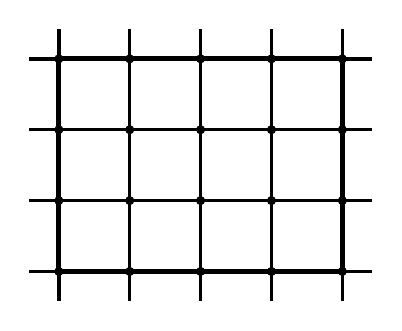
\begin{tikzpicture}[scale=0.75]
  % --- grid size (number of cells) ---
  \def\Nx{4}    % columns of cells
  \def\Ny{3}    % rows of cells
  \def\s{1.2}   % spacing
  \def\ext{0.5}% overshoot amount (in same units as coords)

  % --- draw vertical lines with overshoot ---
  \foreach \i in {0,...,\Nx} {
    \draw[line width=1.2pt]
      (\i*\s,-\ext) -- (\i*\s,\Ny*\s+\ext);
  }

  % --- draw horizontal lines with overshoot ---
  \foreach \j in {0,...,\Ny} {
    \draw[line width=1.2pt]
      (-\ext,\j*\s) -- (\Nx*\s+\ext,\j*\s);
  }

  % --- outer boundary (frame) ---
  \draw[line width=1.8pt] (0,0) rectangle (\Nx*\s,\Ny*\s);

  % --- dots at each intersection (inside the frame) ---
  \foreach \i in {0,...,\Nx} {
    \foreach \j in {0,...,\Ny} {
      \fill (\i*\s,\j*\s) circle (2.2pt);
    }
  }
\end{tikzpicture}
\end{center}

Edges $E$, Vertices $V$, Faces/Plaquette $F/P$;
The qubits be on edges. \\
Periodic boundary conditions = toric code \\
Planar = surface code \\
The goal of all of these constructions is to find a way to represent a stabilizer state, meaning we can write down a series of stabilizer generators which all commute with each other. (This is the fun game with simple rules - just find a systematic way of getting a bunch of stuff commuting and we get a code.) \\

The state generator which will be the products around the edges corresponds to the vertex $v$
\begin{equation}
    A_v = \prod_{e \sim v} X_e \text{ and } B_p =  \prod_{e \sim f} Z_e
\end{equation}

\begin{center}
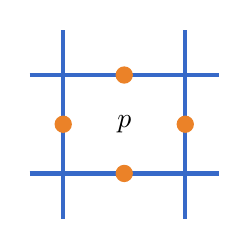
\begin{tikzpicture}[scale=0.5]
  % colors close to the figure
  \definecolor{lineblue}{RGB}{55,105,200}
  \definecolor{dotorange}{RGB}{235,130,40}

  % parameters
  \def\L{2.4}     % half-length of each long line segment
  \def\xs{1.55}   % x-position of the two vertical grid lines
  \def\ys{1.25}   % y-position of the two horizontal grid lines
  \def\r{0.22}    % dot radius

  % grid lines (2 vertical + 2 horizontal)
  \draw[line width=1.5pt, lineblue] (-\xs,-\L) -- (-\xs,\L);
  \draw[line width=1.5pt, lineblue] ( \xs,-\L) -- ( \xs,\L);
  \draw[line width=1.5pt, lineblue] (-\L,-\ys) -- (\L,-\ys);
  \draw[line width=1.5pt, lineblue] (-\L, \ys) -- (\L, \ys);

  % dots (midpoints of each side of the central square)
  \fill[dotorange, line width=1.5pt] (0, \ys)  circle (\r);   % top
  \fill[dotorange, line width=1.5pt] (0,-\ys)  circle (\r);   % bottom
  \fill[dotorange,  line width=1.5pt] (-\xs,0)  circle (\r);   % left
  \fill[dotorange, line width=1.5pt] ( \xs,0)  circle (\r);   % right

  % label
  \node at (0,0) {$p$};
\end{tikzpicture}
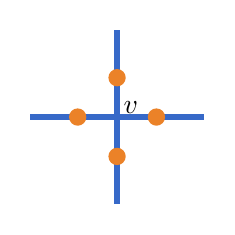
\begin{tikzpicture}[scale=0.5]
  % colors
  \definecolor{lineblue}{RGB}{55,105,200}
  \definecolor{dotorange}{RGB}{235,130,40}

  % parameters
  \def\L{2.2}   % half-length of the cross arms
  \def\r{0.22}  % radius of the dots

  % cross
  \draw[line width=2pt, lineblue] (-\L,0) -- (\L,0);
  \draw[line width=2pt, lineblue] (0,-\L) -- (0,\L);

  % dots (top, bottom, left, right)
  \fill[dotorange,  line width=1.5pt] (0, 1.0) circle (\r);
  \fill[dotorange, line width=1.5pt] (0,-1.0) circle (\r);
  \fill[dotorange, line width=1.5pt] (-1.0,0) circle (\r);
  \fill[dotorange, line width=1.5pt] ( 1.0,0) circle (\r);

  % label
  \node at (0.35,0.25) {$v$};
\end{tikzpicture}
\end{center}